\documentclass[journal,12pt,twocolumn]{IEEEtran}

\usepackage{setspace}
\usepackage{gensymb}

\singlespacing


\usepackage[cmex10]{amsmath}

\usepackage{amsthm}

\usepackage{mathrsfs}
\usepackage{txfonts}
\usepackage{stfloats}
\usepackage{bm}
\usepackage{cite}
\usepackage{cases}
\usepackage{subfig}

\usepackage{longtable}
\usepackage{multirow}

\usepackage{enumitem}
\usepackage{mathtools}
\usepackage{steinmetz}
\usepackage{tikz}
\usepackage{circuitikz}
\usepackage{verbatim}
\usepackage{tfrupee}
\usepackage[breaklinks=true]{hyperref}
\usepackage{graphicx}
\usepackage{tkz-euclide}
\usepackage{float}

\usetikzlibrary{calc,math}
\usepackage{listings}
    \usepackage{color}                                            %%
    \usepackage{array}                                            %%
    \usepackage{longtable}                                        %%
    \usepackage{calc}                                             %%
    \usepackage{multirow}                                         %%
    \usepackage{hhline}                                           %%
    \usepackage{ifthen}                                           %%
    \usepackage{lscape}     
\usepackage{multicol}
\usepackage{chngcntr}

\DeclareMathOperator*{\Res}{Res}

\renewcommand\thesection{\arabic{section}}
\renewcommand\thesubsection{\thesection.\arabic{subsection}}
\renewcommand\thesubsubsection{\thesubsection.\arabic{subsubsection}}

\renewcommand\thesectiondis{\arabic{section}}
\renewcommand\thesubsectiondis{\thesectiondis.\arabic{subsection}}
\renewcommand\thesubsubsectiondis{\thesubsectiondis.\arabic{subsubsection}}


\hyphenation{op-tical net-works semi-conduc-tor}
\def\inputGnumericTable{}                                 %%

\lstset{
%language=C,
frame=single, 
breaklines=true,
columns=fullflexible
}
\begin{document}
\newtheorem{theorem}{Theorem}[section]
\newtheorem{problem}{Problem}
\newtheorem{proposition}{Proposition}[section]
\newtheorem{lemma}{Lemma}[section]
\newtheorem{corollary}[theorem]{Corollary}
\newtheorem{example}{Example}[section]
\newtheorem{definition}[problem]{Definition}

\newcommand{\BEQA}{\begin{eqnarray}}
\newcommand{\EEQA}{\end{eqnarray}}
\newcommand{\define}{\stackrel{\triangle}{=}}
\bibliographystyle{IEEEtran}
\providecommand{\mbf}{\mathbf}
\providecommand{\pr}[1]{\ensuremath{\Pr\left(#1\right)}}
\providecommand{\qfunc}[1]{\ensuremath{Q\left(#1\right)}}
\providecommand{\sbrak}[1]{\ensuremath{{}\left[#1\right]}}
\providecommand{\lsbrak}[1]{\ensuremath{{}\left[#1\right.}}
\providecommand{\rsbrak}[1]{\ensuremath{{}\left.#1\right]}}
\providecommand{\brak}[1]{\ensuremath{\left(#1\right)}}
\providecommand{\lbrak}[1]{\ensuremath{\left(#1\right.}}
\providecommand{\rbrak}[1]{\ensuremath{\left.#1\right)}}
\providecommand{\cbrak}[1]{\ensuremath{\left\{#1\right\}}}
\providecommand{\lcbrak}[1]{\ensuremath{\left\{#1\right.}}
\providecommand{\rcbrak}[1]{\ensuremath{\left.#1\right\}}}
\theoremstyle{remark}
\newtheorem{rem}{Remark}
\newcommand{\sgn}{\mathop{\mathrm{sgn}}}
\providecommand{\abs}[1]{\left\vert#1\right\vert}
\providecommand{\res}[1]{\Res\displaylimits_{#1}} 
\providecommand{\norm}[1]{\left\lVert#1\right\rVert}
%\providecommand{\norm}[1]{\lVert#1\rVert}
\providecommand{\mtx}[1]{\mathbf{#1}}
\providecommand{\mean}[1]{E\left[ #1 \right]}
\providecommand{\fourier}{\overset{\mathcal{F}}{ \rightleftharpoons}}
%\providecommand{\hilbert}{\overset{\mathcal{H}}{ \rightleftharpoons}}
\providecommand{\system}{\overset{\mathcal{H}}{ \longleftrightarrow}}
	%\newcommand{\solution}[2]{\textbf{Solution:}{#1}}
\newcommand{\solution}{\noindent \textbf{Solution: }}
\newcommand{\cosec}{\,\text{cosec}\,}
\providecommand{\dec}[2]{\ensuremath{\overset{#1}{\underset{#2}{\gtrless}}}}
\newcommand{\myvec}[1]{\ensuremath{\begin{pmatrix}#1\end{pmatrix}}}
\newcommand{\mydet}[1]{\ensuremath{\begin{vmatrix}#1\end{vmatrix}}}
\numberwithin{equation}{subsection}
\makeatletter
\@addtoreset{figure}{problem}
\makeatother
\let\StandardTheFigure\thefigure
\let\vec\mathbf
\renewcommand{\thefigure}{\theproblem}
\def\putbox#1#2#3{\makebox[0in][l]{\makebox[#1][l]{}\raisebox{\baselineskip}[0in][0in]{\raisebox{#2}[0in][0in]{#3}}}}
     \def\rightbox#1{\makebox[0in][r]{#1}}
     \def\centbox#1{\makebox[0in]{#1}}
     \def\topbox#1{\raisebox{-\baselineskip}[0in][0in]{#1}}
     \def\midbox#1{\raisebox{-0.5\baselineskip}[0in][0in]{#1}}
\vspace{3cm}
\title{ASSIGNMENT 2}
\author{B.SandhyaRani}
\maketitle
\newpage
\bigskip
\renewcommand{\thefigure}{\theenumi}
\renewcommand{\thetable}{\theenumi}
Download all python codes from 
\begin{lstlisting}
https://github.com/balumurisandhyarani550/ASSIGNMENT2/tree/main/ASSIGNMENT4/CODES
\end{lstlisting}
%
and latex-tikz codes from 
%
\begin{lstlisting}
https://github.com/balumurisandhyarani550/ASSIGNMENT2/tree/main/ASSIGNMENT4
\end{lstlisting}
%
\section{Question No 2.8}
Which of the following pairs of linear equations are consistent/inconsistent, obtain the solution:
%
\begin{enumerate}
%\begin{multicols}{2}
\item
\begin{align}
\begin{split}
\myvec{1 & 1 }\vec{x}&=5
\\
\myvec{2 & 2 }\vec{x}&=10 \label{1.0.1}
\end{split}
\end{align}
\item
\begin{align}
\begin{split}
\myvec{1 & -1 }\vec{x}&=8
\\
\myvec{3 & -3 }\vec{x}&=16 \label{1.0.2}
\end{split}
\end{align}
%\end{multicols}
\end{enumerate}
%
\section{SOLUTION}  
\begin{enumerate}
\item
\begin{align}
\begin{split}
\myvec{1 & 1 }\vec{x}&=5
\\
\myvec{2 & 2 }\vec{x}&=10
\end{split}
\end{align}
The above equations can be expressed as the matrix equation
\begin{align}
\myvec{1 & 1\\2 & 2} \vec{x} = \myvec{5\\10}
\end{align}
%
The augmented matrix for the above equation is row reduced as follows
\begin{align}
\myvec{1 & 1 & 5\\2 & 2 & 10} 
\xleftrightarrow {R_2\leftarrow R_2 -2R_1}\myvec{1 & \ 1 & 5 \\0 & 0 & 0 }
\end{align}
%
$\because$ row reduction of the $2\times 3$ matrix
%
\begin{align}
\myvec{1 & 1 & 5\\0 & 0 & 0} 

\end{align}
%
results in a matrix with 1 nonzero row, its rank is 1. 
%
Similarly, the rank of the matrix 
\begin{align}
\myvec{1 & 1 \\2 & 2 } 
\end{align}
%
is also 1.
%
\begin{align}
\because Rank \myvec{1 & 1\\2 & 2} &= Rank\myvec{1 & 1 & 5\\2 & 2 & 10} \nonumber\\
 &=dim \myvec{1 & 1\\2 & 2}\nonumber\\
 &=1
\end{align}
$\therefore$ Given lines \eqref{1.0.1} have infinitely many solutions so we can say they concide. The given lines are consistent. 
\item
\begin{align}
\begin{split}
\myvec{1 & -1 }\vec{x}&=8  
\\
\myvec{3 & -3 }\vec{x}&=16
\end{split}
\end{align}
The above equations can be expressed as the matrix equation
\begin{align}
\myvec{1 & -1\\3 & -3}
//
\vec{x} = \myvec{8\\16}
\end{align}
%
The augmented matrix for the above equation is row reduced as follows
\begin{align}
\myvec{1 & -1 & 8\\3 &-3 & 16 }
\xleftrightarrow {R_2\leftarrow R_2-3R_1}\myvec{1 & -1 & 8 \\0 & 0 & -8}
\\
\end{align}
%
$\because$ row reduction of the $2\times 3$ matrix
%
\begin{align}
\myvec{1 & -1 & 8\\3 & -3 & 16}
\end{align}
%
results in a matrix with 2 nonzero rows, its rank is 2. 
%
Similarly, the rank of the matrix 
\begin{align}
\myvec{1 & -1 \\3 & -3 } 
\end{align}
%
is also 1.
%
\begin{align}
\because Rank \myvec{1 & -1\\3 & -3} \ne Rank\myvec{1 & -1 & 8\\3 & -3 & 16}\nonumber\\
\end{align}
$\therefore$ Given lines \eqref{1.0.2} have no solution so we say they are parallel. The givens lines are inconsistent. 
PLOT OF GIVEN LINES -
\numberwithin{figure}{section}
\begin{figure}[ht!]
Plot of \eqref{1.0.1} -
    \centering
    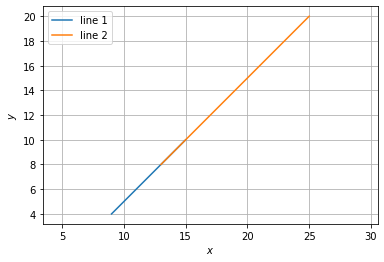
\includegraphics[width=\columnwidth]{consistent.png}
    \caption{SAME LINES}
    \label{fig:SAME LINES.}
\end{figure} 
\numberwithin{figure}{section}
\begin{figure}[ht]
Plot of \eqref{1.0.2} 
    \centering
   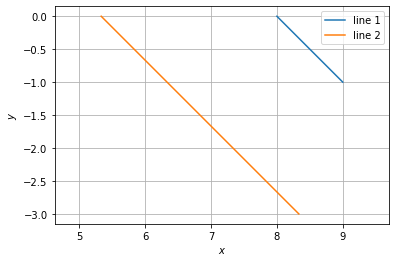
\includegraphics[width=\columnwidth]{inconsistent.png}
    \caption{Parallel lines}
    \label{fig: PARALLEL lines.}
\end{figure}    
\end{enumerate}
\end{document}